\subsubsection{Desarrollo de mecanismos de autenticación}

La autenticación es una de las funciones más críticas en el sistema, ya que asegura que los usuarios solo puedan acceder a la aplicación con credenciales válidas en el AD. A continuación, se describen los mecanismos de autenticación desarrollados, destacando las interacciones con el AD y el uso de tokens para la gestión de sesiones.

\textbf{Manejadores de autenticación}

Como se explicó en secciones anteriores, los manejadores (handlers) authenticationSetHandler (\autoref{fig:authentication-set-handler})  y ldapUnbindHandler (\autoref{fig:ldap-unbind-handler}) juegan un papel crucial en la gestión de la autenticación. Estos aseguran que las conexiones al AD se establezcan y se liberen correctamente tras cada solicitud, manteniendo el sistema seguro y eficiente.

\textbf{Proceso de inicio de sesión}

El proceso de autenticación se basa en la operación \textbf{bind} proporcionada por el cliente LDAP. Este proceso se gestiona en el módulo de autenticación, método \textbf{signIn}, encargado de validar las credenciales del usuario y establecer las cookies de sesión. En la \autoref{fig:flow-diagram-auth-method} se muestra el diagrama de flujo detallando los pasos seguidos por el método:
\begin{enumerate}
    \item \textbf{Validación del formulario y captcha}: El sistema recibe los datos del formulario de inicio de sesión y valida tanto las credenciales del usuario como el token de captcha para prevenir intentos de acceso automatizados y ataques de fuerza bruta.
    \item \textbf{Autenticación en el AD}: Una vez que el captcha y las credenciales del usuario se validan correctamente, el sistema intenta autenticar al usuario en el AD a través del cliente LDAP. Si la autenticación falla, se maneja de acuerdo con los diferentes códigos de error que proporciona el AD, permitiendo mensajes de error detallados como "Credenciales inválidas", "Cuenta deshabilitada", o "Contraseña expirada".
    \item \textbf{Generación de tokens y cookies}: Si la autenticación es exitosa, el sistema recupera la entrada del usuario en el AD y genera los tokens de sesión y acceso. Estos tokens se almacenan en cookies para futuras solicitudes.
    \item \textbf{Redirección del usuario}: Una vez completado el proceso de inicio de sesión, el sistema redirige al usuario a su página de perfil.
\end{enumerate}

\begin{figure}[H]
    \centering
    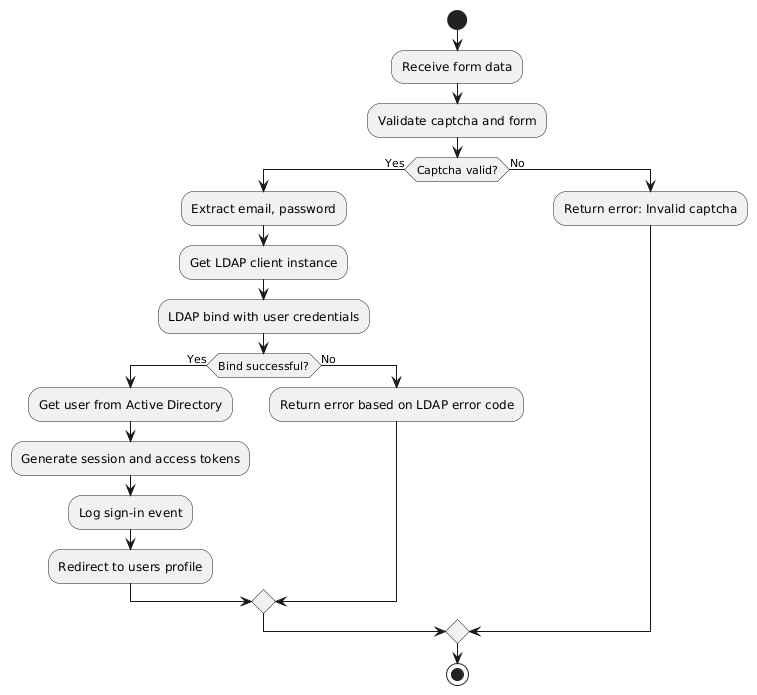
\includegraphics[scale=0.5]{images/puml/flow-diagram-signin/flow-diagram signin.png}
    \caption{Diagrama de flujo: Función de autenticación}
    \label{fig:flow-diagram-auth-method}
\end{figure}

\textbf{Proceso de cierre de sesión}

Este proceso se gestiona en el módulo de autenticación, método signOut, que elimina las cookies de sesión y acceso, invalidando así la sesión del usuario. Este mecanismo asegura que, tras cerrar la sesión, el usuario ya no podrá acceder a la aplicación hasta que vuelva a autenticarse correctamente (\autoref{fig:flow-diagram-signout-method}).

\begin{figure}[H]
    \centering
    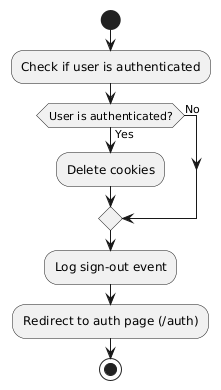
\includegraphics[scale=0.6]{images/puml/flow-diagram-signout/flow-diagram signout.png}
    \caption{Diagrama de flujo: Función cerrar sesión}
    \label{fig:flow-diagram-signout-method}
\end{figure}
